\documentclass{beamer}
%\usepackage[latin1]{inputenc}

\usepackage[utf8]{inputenc}
\usepackage{polski}
\usepackage{graphicx}

\usetheme{Warsaw}
\title[Sieci Bayesowskie]{Uczenie modeli kanonicznych w sieciach Bayesowskich - efektywne uczenie modelu Noisy OR/MAX z danych}
\author{Krzysztof Nowak}
\institute{Politechnika Białostocka}
\date{23.10.2012}
\begin{document}

\begin{frame}
\titlepage
\end{frame}

\begin{frame}{Wprowadzenie}
	Sieć Bayesowska - struktura służąca do przedstawiania zależności pomiędzy zdarzeniami, bazując na rachunku prawdopodobieństwa.


	\pause W sieciach bayesowskich można wyróżnić:
	\begin{itemize}
		\pause \item Strukturę sieci - skierowany, acykliczny graf
		\pause \item Parametry sieci - wartości liczbowe określające prawdopodobieństwo poszczególnych zdarzeń
	\end{itemize}
	
\end{frame}

\begin{frame}{Struktura sieci}
	\begin{figure}[h!]
		\centering
		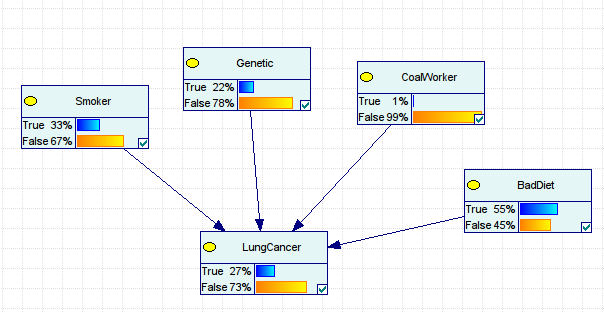
\includegraphics[width=10cm]{1.png}
		\caption{Przykładowa sieć bayesowska - Genie 2.0}
	\end{figure}
\end{frame}

\begin{frame}{Parametry sieci}
	CPT - Conditional Probability Table
	\begin{figure}[h!]
		\centering
		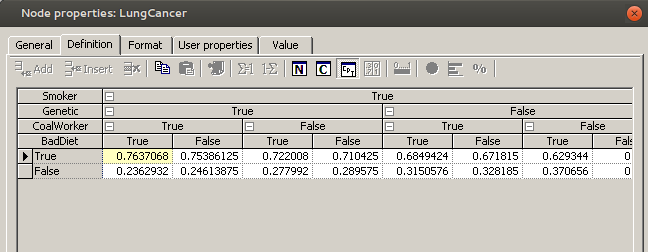
\includegraphics[width=10cm]{2.png}
		\caption{CPT - Genie 2.0}
	\end{figure}
	\begin{itemize}
		\item Wykładniczy przyrost parametrów ze względu na ilość węzłów rodzicielskich.
		\item Przydatny model przy uczeniu sieci z dużych zbiorów danych.
	\end{itemize}
\end{frame}

\begin{frame}{Parametry sieci}
	\begin{figure}[h!]
		\centering
		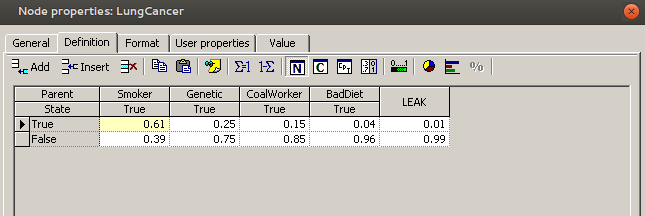
\includegraphics[width=10cm]{3.png}
		\caption{Noisy MAX/OR - Genie 2.0}
	\end{figure}

	\begin{itemize}
		\item Liniowy przyrost parametrów ze względu na ilość węzłów rodzicielskich.
		\item Przydatny model przy uczeniu sieci z małych zbiorów danych, bądź wiedzy eskperta.
		\item Bramka Noisy OR jest szczególnym przypadkiem bramki Noisy MAX.
	\end{itemize}
\end{frame}

\begin{frame}{Modele kanoniczne - Noisy OR}
	\begin{itemize}
		\item Najprostszy i najbardziej intuicyjny z modeli kanonicznych.
	\end{itemize}
	Bramka Noisy-OR wymaga podania prawdopodobieństwa wystąpienia danego zjawiska dla poszczególnych wartości węzłów rodzicielskich, niezależnie od pozostałych:
	\begin{equation}
		p_k = P(y|\bar{x}_1, \bar{x}_2, ... , x_k, ... , \bar{x}_{n-1}, \bar{x}_n).
	\end{equation}
	Prawdopodobieństwo w bramce Noisy-OR przy wektorze wejściowym $\textbf{X}$ wyliczamy następująco:
	\begin{equation}
		P(y|\textbf{X}) = 1 - \prod_{i:x_i\epsilon \textbf{X}}(1-p_i)
	\end{equation}

	Parametr ``LEAK'' oznacza prawdopodobieństwo wystąpienia danego zjawiska, pomimo braku wystąpienia jakiejkolwiek jawnej przyczyny. 
	Służy on do uwzględnienia tzw. niewymodelowanych przypadków:

	\begin{equation}
		p_{leak} = P(y|\bar{x}_1, \bar{x}_2, ... , \bar{x}_n).
	\end{equation}
\end{frame}

\begin{frame}{Wyliczanie parametrów z danych - CPT}
	Standardowy węzeł w sieci bayesowskiej wymaga podania całej tabeli prawdopodobieństw warunkowych. 
	Zliczamy poszczególne wystąpienia danych kombinacji parametrów w pliku z danymi i na ich podstawie wyliczamy prawdopodobieństwo.

	\begin{figure}[h!]
		\centering
		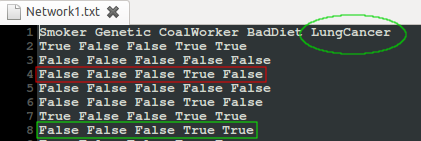
\includegraphics[width=10cm]{4.png}
		\caption{Przykładowy plik z danymi}
	\end{figure}
	\begin{equation}
	\frac{\textcolor{green}{27}}{\textcolor{green}{27} + \textcolor{red}{311}} = 0.079
	\end{equation}
\end{frame}	
\begin{frame}{Wyliczanie parametrów z danych - Noisy-OR/MAX}
	\begin{itemize}
		\item Węzeł typu Noisy-OR/MAX nie wymaga podania prawdopodobieństwa dla każdej możliwej kombinacji parametrów, a jedynie dla prawdopodobieństwa wystąpienia każdego z parametrów z osobna (niezależnie od innych).
		\item Sposób wyliczania jest identyczny, jednak ze względu na charakter bramki Noisy-OR/MAX potrzebujemy znacznie mniej parametrów.
	\end{itemize}
\end{frame}

\begin{frame}{Usprawnienie wyliczania parametrów z danych - Noisy-OR/MAX}
	\begin{itemize}
		\item W podanym wcześniej pliku z danymi, ilość rekordów składających się na wyliczenie wszystkich parametrów dla bramki Noisy-OR to około \textbf{47\%} wszystkich rekordów.
		\item Można to interpretować w taki sposób: Przy określaniu parametrów dla bramki Noisy-OR, pomijamy około \textbf{53\%} informacji zawartych w danych.
		\item Dla porównania, określenie parametrów (CPT) dla bramki standardowej wykorzystuje cały plik z danymi.
		\pause \item Czy da się lepiej uzyskać poszczególne parametry sieci Noisy-OR ?
	\end{itemize}
\end{frame}

\begin{frame}{Usprawnienie wyliczania parametrów z danych.}
	\begin{itemize}
		\item Układy równań parametrów.
		\pause \item Zamiast zliczać rekordy w danych określające każdy z parametrów bezpośrednio (Noisy-OR), wybieramy $n$ kombinacji o największej liczbie ``reprezentantów'' w danych.
		\pause \item Otrzymujemy w ten sposób pewien zbiór kombinacji parametrów, przykładowo:

			$x_1, \bar{x_2}, x_3, \bar{x_4} = p_{1,3}$

			$x_1, \bar{x_2}, \bar{x_3}, x_4 = p_{1,4}$

			$\bar{x_1}, \bar{x_2}, x_3, x_4 = p_{3,4}$

			$x_1, x_2, x_3, \bar{x_4} = p_{1,2,3}$
		\pause \item Zależy nam na uzyskaniu parametrów $p_1, p_2, p_3, p_4$.
	\end{itemize}
\end{frame}

\begin{frame}{Rozwiązywanie układu równań}
	\begin{itemize}
		\item Korzystając ze wzoru (2) mamy:

		$1 - (1-p_1)\times(1-p_3) = p_{1,3}$

		$1 - (1-p_1)\times(1-p_4) = p_{1,4}$

		$1 - (1-p_3)\times(1-p_4) = p_{3,4}$

		$1 - (1-p_1)\times(1-p_2)\times(1-p_3) = p_{1,2,3}$

		\pause \item Aby uprościć obliczenia, rozwiązujemy układ dla $1-p_i$ zamiast $p_i$ (używamy podstawienia $p'_i = 1 - p_i$).
		\pause
		$1 - (p`_1)\times(p`_3) = p_{1,3}$

		$1 - (p`_1)\times(p`_4) = p_{1,4}$

		$1 - (p`_3)\times(p`_4) = p_{3,4}$

		$1 - (p`_1)\times(p`_2)\times(p`_3) = p_{1,2,3}$
	\end{itemize}
\end{frame}

\begin{frame}{Rozwiązywanie układu równań}
	\begin{itemize}
	\item
		Ostatecznie otrzymujemy:

		$(p`_1)\times(p`_3) = 1 - p_{1,3}$

		$(p`_1)\times(p`_4) = 1 - p_{1,4}$

		$(p`_3)\times(p`_4) = 1 - p_{3,4}$

		$(p`_1)\times(p`_2)\times(p`_3) = 1 - p_{1,2,3}$
	\item Nie jest to liniowy układ równań. 
	\begin{enumerate}
		\item Rozwiązanie za pomocą zmodyfikowanej eliminacji gaussa.
		\item Zlogarytmować obustronnie każde z równań.
	\end{enumerate}
		
		$\log{(p`_1)} + \log{(p`_3)} = \log{(1 - p_{1,3}) }$

		$\log{(p`_1)} + \log{(p`_4)} = \log{(1 - p_{1,4}) }$

		$\log{(p`_3)} + \log{(p`_4)} = \log{(1 - p_{3,4}) }$

		$\log{(p`_1)} + \log{(p`_2)} + \log{(p`_3)} = \log{(1 - p_{1,2,3}) }$

	\end{itemize}
\end{frame}

\begin{frame}{Rozwiązywanie układu równań}
	\begin{itemize}
		\item Uzyskane w ten sposób parametry $p''_i = \log{(p'_i)}$ dają nam szukane parametry $p_i$ przez ponowne podstawienie: 

		$p_i = 1 - e^{p''_i}$, gdzie e - podstawa logarytmu (dowolna)

		\item Rozwiązanie samego układu nie stanowi problemu
		\item Wybór odpowiednich równań jest kluczowy - Równania muszą być liniowo niezależne
		\item Sam wybór stanowi o skuteczności ostatecznego rozwiązania:
		\begin{enumerate}
			\item Optymalizacja sumarycznej ilości ``reprezentatów'' w układzie równań. 
			\item Rozwiązanie $n$ układów, rozpatrując każdy z parametrów z osobna.
			\item Rozwiązanie $m$ układów równań, i wyliczenie $m$ zestawów parametrów, z których wyliczamy ostateczny zestaw parametrów za pomocą średniej ważonej.
		\end{enumerate}
	\end{itemize}
	Przydatna będzie heurystyka wyboru równań uwzględniającą ich liniową niezależność. Dokładne rozwiązanie może być złożone ${2^n \choose n}$.
\end{frame}

\begin{frame}{Wyniki}
	\begin{figure}[h!]
		\centering
		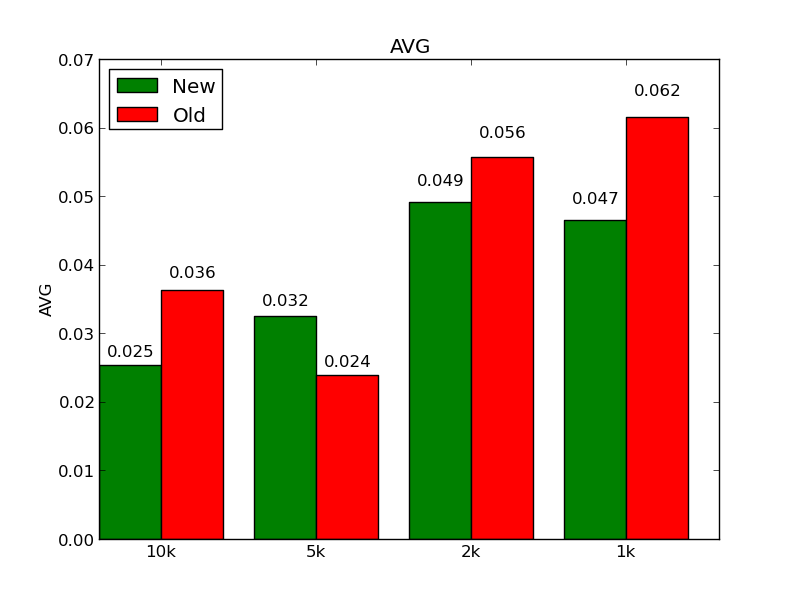
\includegraphics[width=9cm]{avg.png}
		\caption{Średni błąd parametru}
	\end{figure}
\end{frame}

\begin{frame}{Wyniki}
	\begin{figure}[h!]
		\centering
		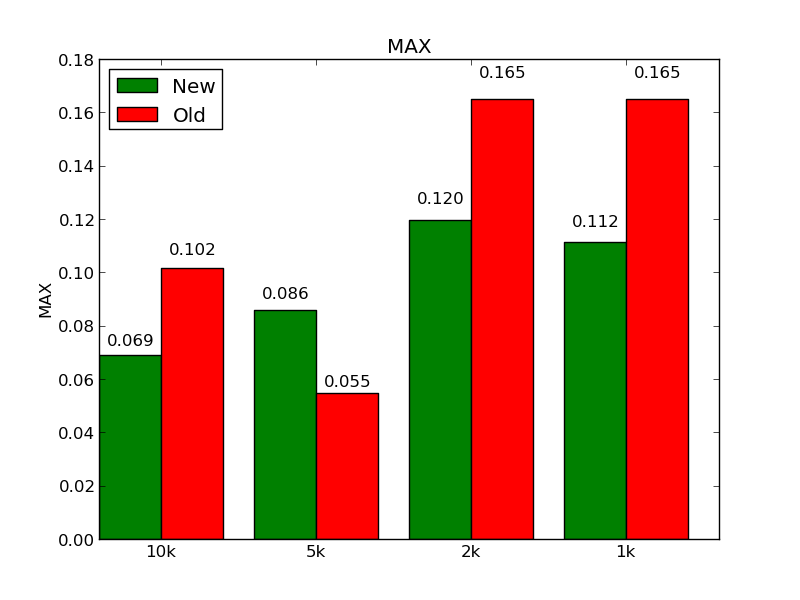
\includegraphics[width=9cm]{max.png}
		\caption{Maksymalny błąd parametru}
	\end{figure}
\end{frame}

\begin{frame}{Wyniki}
	\begin{figure}[h!]
		\centering
		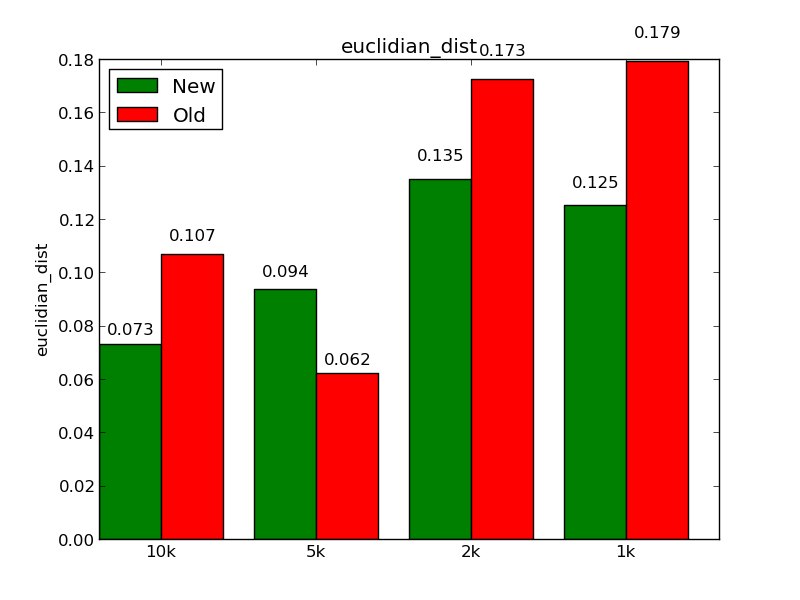
\includegraphics[width=9cm]{euclidian_dist.png}
		\caption{Odległość euklidesowa.}
	\end{figure}
\end{frame}

\begin{frame}{Wyniki}
	\begin{figure}[h!]
		\centering
		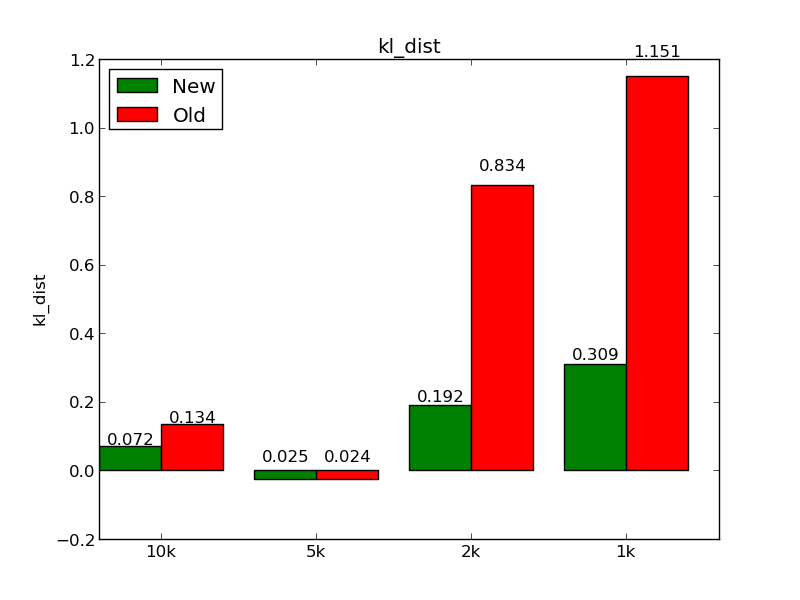
\includegraphics[width=9cm]{kl_dist.png}
		\caption{Dywergencja Kullbacka-Leiblera.}
	\end{figure}
\end{frame}

\begin{frame}{Wyniki}
	\begin{figure}[h!]
		\centering
		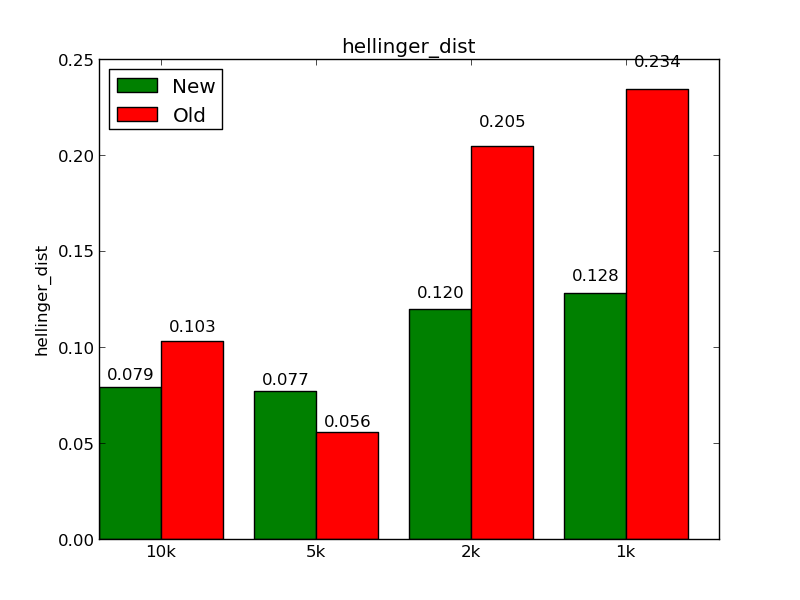
\includegraphics[width=9cm]{hellinger_dist.png}
		\caption{Odległość Hellingera.}
	\end{figure}
\end{frame}



\begin{frame}{Źródła}
	\begin{itemize}
		\item Francisco J. Diez, Marek J. Drużdżel - "Canonical Probabilistic Models for Knowledge Engineering" (28.4.2007)
		\item Nir Friedman, Moises Goldszmidt - "Learning Bayesian networks with local structure"
		\item Agnieszka Oniśko, Marek J. Drużdżel, Hanna Wasyluk - "Learning Bayesian network parameters from small data sets: application of Nosiy-OR gates" (1.3.2001)
	\end{itemize}
\end{frame}
\end{document}
